\documentclass{article}

\usepackage{amsmath}
\usepackage{graphicx}
\usepackage[a4paper, margin=0.5in]{geometry} % Adjusts margin size

% \usepackage{natbib}

\title{Homework 7 — pdf portion} 
\author{Christian Burt\\ASTR 400B}
\date{March 28, 2025}

% The preamble ends with the command \begin{document}
\begin{document}
\maketitle
\setcounter{section}{4} % Section counter += 4
    
    \section{Questions}

    \begin{enumerate}

    % \setcounter{enumi}{1} % += 1
    \item 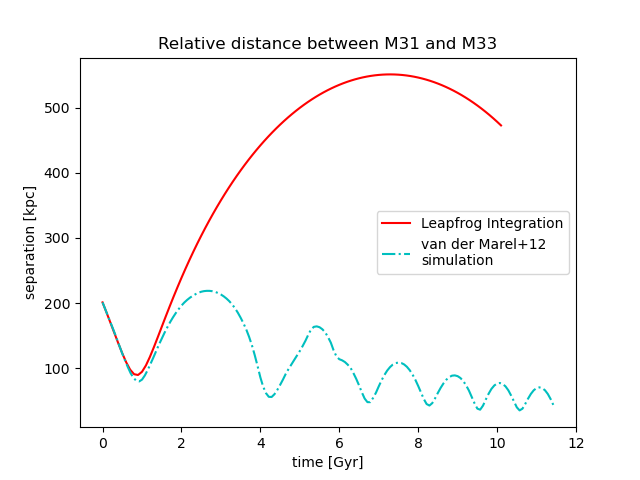
\includegraphics[width=0.5\linewidth]{M33-M31-rel-pos.png}
      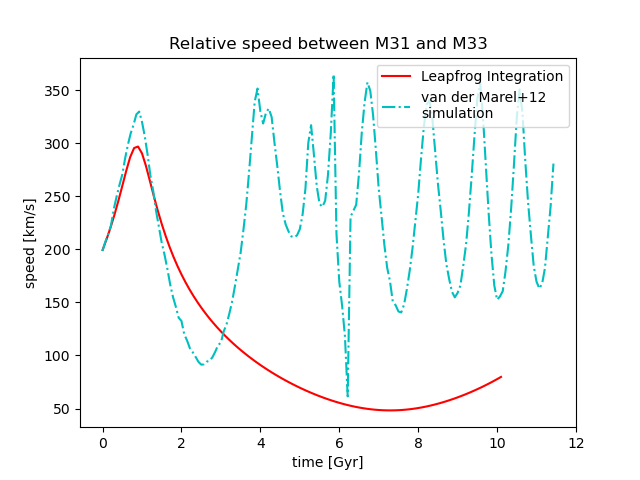
\includegraphics[width=0.5\linewidth]{M33-M31-rel-vel.png}

    \item The leapfrog simulation conducted assuming point-like
      galaxies witnessed one close encounter before rapidly receding
      from one another, similar to the orbit of binary stars with a
      high ellipticity. At around $7\,\,\text{Gyr}$, in the future, the galaxies
      briefly stop relative to one another and begin moving towards
      each other.
      
      Meanwhile, the N-body simulation begins
      similarly, but depicts an orbit that is decaying with five close
      encounters within $10\,\,\text{Gyr}$ and an ever decreasing aphelion.

      The velocity plots corroborate this, with the Leapfrog
      integrator showing one velocity spike at the close encounter
      before racing away and eventually stopping and
      returning. Meanwhile, the N-body simulation plots a much more
      sporatic speed evolution.
      
    \item As I mentioned in the previous question, our point-like
      acceleration method assumes galaxies operate like compact
      binaries or a planetary orbit. This approximation is useful when
      the center of mass of the galaxies is far, but during the first
      close encounter, the gravitational force between individual
      stars and halo particles in each galaxy becomes significant,
      greatly reducing the relative velocity between each galaxy in a
      processes called dynamical friction.
      
    \item To consider MW in our leapfrog orbital integrator, we would
      need to consider the acceleration between MW and M31 as well as
      the acceleration between M33. This would have the effect of
      creating a 3-body simulation. Note that since MW and M31 would
      behave like point-like particles, they would not merge as we
      expect, so this simulation would also predict a very different
      result from the individual particle simulation.

    \end{enumerate}

\end{document}
